% TEMPLATE for Usenix papers, specifically to meet requirements of
%  USENIX '05
% originally a template for producing IEEE-format articles using LaTeX.
%   written by Matthew Ward, CS Department, Worcester Polytechnic Institute.
% adapted by David Beazley for his excellent SWIG paper in Proceedings,
%   Tcl 96
% turned into a smartass generic template by De Clarke, with thanks to
%   both the above pioneers
% use at your own risk.  Complaints to /dev/null.
% make it two column with no page numbering, default is 10 point

% Munged by Fred Douglis <douglis@research.att.com> 10/97 to separate
% the .sty file from the LaTeX source template, so that people can
% more easily include the .sty file into an existing document.  Also
% changed to more closely follow the style guidelines as represented
% by the Word sample file. 

% Note that since 2010, USENIX does not require endnotes. If you want
% foot of page notes, don't include the endnotes package in the 
% usepackage command, below.

% This version uses the latex2e styles, not the very ancient 2.09 stuff.

% NOTE: use end-notes, not footnotes
%Citation example:
%Now we're going to cite somebody.  Watch for the cite tag.
%Here it comes~\cite{Chaum1981,Diffie1976f}.  The tilde character (\~{})
%in the source means a non-breaking space.  This way, your reference will
%always be attached to the word that preceded it, instead of going to the
%next line.

\documentclass[letterpaper,twocolumn,10pt]{article}
\usepackage{usenix,epsfig,graphicx,float,url,longtable}
\newcommand{\comment}[1]{}
%\newcommand{\Syndicate}{Obfuscate}
\newcommand{\Syndicate}{Syndicate}
\begin{document}

%don't want date printed
\date{}

%make title bold and 14 pt font (Latex default is non-bold, 16 pt)
\title{\Large \bf \Syndicate: Delivering Durable and Scalable Storage\\ Through Service Composition}

%for single author (just remove % characters)
\author{
%{\rm Paper \#152}\\
%\and
%{\rm Pages: 14}\\
% copy the following lines to add more authors
 {\rm Jude Nelson}\\
Princeton University
 \and
 {\rm Larry Peterson}\\
Princeton University
} % end author

\maketitle

% Use the following at camera-ready time to suppress page numbers.
% Comment it out when you first submit the paper for review.
% \thispagestyle{empty}

\setlength{\parskip}{0pt}
\setlength{\parsep}{0pt}
\setlength{\headsep}{0pt}
\setlength{\topskip}{0pt}
\setlength{\topmargin}{0pt}
\setlength{\topsep}{0pt}
\setlength{\partopsep}{0pt}
	
\subsection*{Abstract}

This paper presents Syndicate, a wide-area distributed filesystem that
delivers high read performance to a scalable number of readers by
leveraging an underlying content distribution network (CDN).
Syndicate is unique in that it separates file persistence from
read performance by leveraging a CDN to drive data distribution
between clients.  In doing so, Syndicate achieves good aggregate
read bandwidth between its clients despite the poor read bandwidth of 
the underlying data storage.  This architecture also allows the system
to achieve good read performance with a scalable number of clients without
requiring clients to replicate data.

Syndicate provides
conventional read/write and access control semantics while guaranteeing
close-to-open consistency. We evaluate the Syndicate prototype with a series of
microbenchmarks using two CDN implementations in which we test Syndicate's
file I/O latency and bandwidth when reading and writing datasets 
and filesystem hierarchies.



\section{Introduction}

Over the past decades, email has gained wide-spread adoption 
and is now a core communication service for society. However, 
some of its original design choices have had a profound impact 
on email information security, email storage, and common email 
tasks like search and filtering. In this paper, we revisit some 
of these choices and propose a backwards-compatible email service, 
called STEAK, that addresses these concerns in the context of 
contemporary usability expectations.

Users send a wide variety of information in their email messages, 
including confidential and personal information and legally-binding 
documents. Traditional email protocols, like SMTP and IMAP, do not 
provide adequate security guarantees and average email users are 
sometimes not even aware that they're communicating over a fundamentally 
insecure channel. In a secure communication channel, when Alice sends 
Bob a message, only Bob can read it (message confidentiality), Bob can 
verify that the message he received was in fact sent by Alice (message 
authenticity), and that it contains the data she sent (message integrity). 
Traditional email protocols provide none of these security properties 
out of the box. 

At the same time, users have come to expect certain features on top of 
traditional email.  These include automatic spam filtering, the ability 
to search and organize messages, and ubiquitous access to their email 
through webmail from a variety of user devices. We believe that providing 
stronger security guarantees cannot come at an expense of reduced usability. 
Our goal is to design an email service that provides the fundamental 
security properties of message confidentiality, integrity, and authenticity 
(called CIA guarantees in the rest of the paper), while providing the 
features and user experience of webmail.  This is a nontrivial problem 
and current security approaches require running out-of-band security 
systems ``on top'' of email usually by leveraging public-key cryptography. 
These include S/MIME and PGP, as well as more recent ID-based encryption 
schemes [ref].

The problem with out-of-band security approaches is that it significantly 
reduces usability by requiring active involvement in key management. 
Users must generate, distribute, and revoke public keys with the out-of-band 
system, and carefully guard their private keys while remaining vigilant 
for compromises. We believe this is unreasonable because most users do 
not understand practical information security, and want the convenience 
of webmail despite the security problems it introduces. Even if they 
understood the security concerns, using public-key cryptography in this 
manner greatly increases the complexity of basic email tasks. 

Our key insight is that email's store-and-forward approach makes CIA 
guarantees hard to achieve. Because each email server stores and processes 
messages, a user must either trust the server completely to not to break 
CIA, or perform end-to-end authenticated encryption outside of the system. 
The former is unrealistic, but the latter requires users to set up and 
manage keys out-of-band. To address these challenges in this paper we 
present a new email system called Security Transparent Email with 
Automatically-managed Keys (STEAK). 

The contributions of STEAK are 1) an automatic key management system 
(called AutoKey) and 2) an email exchange protocol (called Secure Message 
Request Protocol, or SMRP) that allow users to access their email using a 
web browser on any device. STEAK enables access to email with only a 
username/password pair and a small amount of additional logic at the 
email client. To do so, STEAK leverages the user's own personal cloud 
storage to host sealed account state, sealed keys, and sealed messages. 
The user devices (clients), not servers, process messages after decrypting 
them. Within STEAK, the AutoKey system automatically distributes keys, 
e.g., Alice's public keys to Bob, using an array of non-colluding 
repositories. Once keys are distributed, Bob can receive 
messages from Alice using SMRP. Under the hood, SMRP 
actually downloads messages from the sender's cloud storage. All the while, 
STEAK remains transparently backwards-compatible with SMTP, and offers 
a more limited CIA guarantee to non-STEAK users.

The remainder of this paper is organized as follows.  In section ``Motivation'', 
we define our usability requirements, and argue that our strategy is necessary 
to meet them for providing CIA guarantees. Then, we present the design of STEAK 
in section “Design”, with a focus on AutoKey and SMRP, and describe how basic 
email activities are performed.  Afterward, we present our prototype 
implementation (Section “Implementation”), and give a qualitative usability 
analysis and a preliminary performance evaluation (Section “Evaluation”).  
We finish by discussing related and future work (Section “Related and Future 
Work”), and presenting concluding remarks (Section “Conclusion”).

\section{Usage Scenarios}
\label{sec:motivation}

There are many scenarios where users might leverage network caches, local storage, and cloud storage in domain-specific ways.  Rather than build a storage solution from scratch for each scenario, we propose a solution that lets users pick the appropriate infrastructure, while offering reliable set of consistency and durability semantics. The examples motivate such a design. We summarize the requirements at the end of the section.

%The examples are presented from the perspective of users with read/write access to a shared data set, and for readability, they anticipate an idealized version of Syndicate that coordinates access to caches, local storage and cloud storage.

\subsection{Scientific Collaboration}

Thousands of researchers at hundreds of universities often collaborate in the context of large (multi-terabyte) data sets, the GenBank sequencing data being an illustrative example~\cite{GenBank}. These researchers run experiments locally (using local workstations and clusters) on some subset of the larger data set, and then share their preliminary results across the wide-area with collaborators at other universities.  Curators periodically write vetted results back into the core data set, and the cycle continues.

This is difficult to achieve without coordination.  While researchers need to share their latest experimental data sets with many readers in the wide-area, they must also ensure that the readers receive fresh data.  Simply copying the data sets to off-site cloud storage for them to access is a costly and time-consuming process.  Simply serving the data directly from the workstation does not scale.  Employing network caches introduces the possibility of serving stale data.

Under ideal circumstances, researchers would keep data on the local workstations for fast local access (i.e. under interactive settings), and only make back-ups to cloud storage when it is cost-effective to do so.  The workstations could serve recent data to a scalable number of readers if the network caches were guaranteed to only serve data consistent with recent modifications.  However, making this happen requires coordination between the cloud storage provider, the network caches, the workstations, and the wide-area readers.

%Running Syndicate as a local filesystem on each researcher's computer(s) ensure fast local reads of the shared data set and fast local writes of new results, where Syndicate would leverage network caches to efficiently distribute the read-mostly core to thousands of researchers. If a sufficient number of collaborators are interested in a particular researcher's preliminary results, caching will also aid remote reads. If not, readers are still be able to access the latest results directly from the writer's local store.

%GenBank specifically is archived apart from Syndicate (which means Syndicate must import its data to make it available to researchers as a mountable file system), but in general, it would be appropriate to ensure the durability of at least the curated data by having Syndicate replicate it in cloud storage (either public or private).

\subsection{Distributed Authoring and Versioning}

One way to share data in a read/write setting is with distributed authoring and versioning (DAV) servers, such as Apache mod\_dav~\cite{mod_dav}. However, it is difficult to scale the number of readers to a DAV server, while also giving writers the durability they desire.  This is because each writer determines its own remote storage provider for hosting back-ups of its documents, specific to its cost and performance objectives.  All the while, readers must be able to consume data consistent with modifications, even if the DAV server's local storage fails.

Under ideal circumstances, each writer would couple its storage mechanism of choice to the DAV server, such that the DAV server could transparently write modifications to the writer's desired storage.  To ensure a scalable number of readers could receive consistent data, the DAV server would need to replicate the data sufficiently to make it available.  While network caches can do this in read-only settings, the challenge to using them with DAV is to ensure that they serve only consistent data in the face of writes.  This requires coordination between the DAV server, the readers, the writers, and the storage systems.


%With Syndicate, users at the edge can instead deploy their own DAV servers, where each server exposes its locally-hosted documents through a shared Syndicate instance. The DAV servers leverage Syndicate to read data from one another through existing CDNs and network caches, and Syndicate ensures they receive data consistent with recent changes and hit unchanged data in the cache.

%Syndicate lets each user determine the appropriate trade-off between write performance and write durability. If write performance is preferred, only the DAV server stores its users' data, but nevertheless makes it available to all other DAV servers through Syndicate. If write durability is preferred, the DAV server leverages Syndicate to synchronously commit local user data to cloud storage providers that meet the user's cost, performance, and durability requirements.

\subsection{Virtual Desktop Infrastructure}

An alternative approach to supplying employees with corporate computers and smartphones is to let them bring their own hardware, and run a corporate OS in a VM while they are at work. The challenge to doing this at scale is to store and deliver VM images and OS updates to a scalable number of employees across sites, while preserving user sessions in a secure manner.

VM images do not change much between sessions~\cite{collective}, which means unmodified bytes can be cached locally or in intermediate network caches at site peering points. Only modified bytes must be preserved, and each VM image is modified at most one user at a time. Some VDI implementations~\cite{citrix,mokafive} offer implementation-specific caching protocols that leverage these facts.

Ideally, the corporation would choose the cache and storage providers that best meet their business needs.  This may not be the implementation-specific VDI caching mechanism, especially if there already exists proven in-house cache and storage infrastructure.


\subsection{Observations}

These examples show that a user can benefit from storing objects on local storage, or in a remote cloud storage provider. While storing objects locally improves local access performance, it requires the user to take responsibility for object durability, availability, and remote access performance. Storing data objects in the cloud incurs access performance and cost penalties relative to local storage, but gives the objects potentially stronger availability and durability guarantees offered by the cloud storage provider.

In read-heavy settings, network caches become responsible for an object's data read availability instead of the object's origin server. This is because the cost of reading data from an origin server is amortized over many cache hits from many readers, effectively decoupling read performance from write performance and durability. With network caches handling reads, a user can place objects wherever makes sense for the problem domain, even in a last-mile network with limited upload bandwidth.

Regardless of caches, a user trades data write performance for write durability. This is because write durability increases with the number of replicas created, but write performance is only as fast as the slowest storage provider to receive the data. To address this tradeoff, a user chooses which remote storage providers receive written data replicas before a write is said to have completed.

To address read and write performance, a user can host object data locally, but ensure that interested remote readers can discover the data and fetch it via network caches. This is acceptable when there are many readers, because then there is a good chance the requested data will be found in a nearby cache.  The challenge, however, is to ensure that readers discover only fresh data.  This includes ensuring that replicas of local data are consistent, in case the local host fails.

Orthogonal to reads and writes, multiple writers can create multiple objects at once. However, there comes a point in each scenario where there cannot be independent versions of the same object. We address this by ensuring that at all times, a valid object name identifies at most one object.

Although in the abstract all three usage scenarios store and access ``data objcts,'' they each benefit from a different interface: a file system interface in the first example, a web-based service interface in the second example, and a block-level interface in the third example. It's an engineering detail, but ideally the access interface should be decoupled from its core storage capability.


\section{Design}
\label{sec:design}

As described in our motivation, there are two major aspects to STEAK's design.  The first is the subsystem for securely and automatically managing keys.  We refer to this subsystem as AutoKey.  The second is the protocol for sending and receiving emails, called Secure Message Request Protocol (SMRP).  SMRP relies on AutoKey to ensure the sender and receiver have the appropriate keys in place before communicating.

\subsection{Architecture}
Our design assumes Alice and Bob both have sets of trusted endpoints that run loosely-synchronized clocks, For hosting hard state across sessions, we leverage Alice and Bob's personal cloud storage accounts.  Additionally, we assume Alice and Bob's endpoints can run code in execution and resource contexts outside of the web browser (such as in a VM).

There are four components to STEAK, beyond cloud storage and endpoint devices (Figure~\ref{fig:overview}). The first is the STEAK endpoint code, which runs separately from the browser.  It performs key management, session management, caching, cloud storage access, cryptographic operations, and UI proxying. The second is the webmail UI, which differs from a conventional webmail UI only in that it issues its RPCs to the locally-hosted endpoint code instead of a remote webmail server.  These two components are intentionally separated for practical reasons, because at the time of this writing there is no way to perform cryptography inside a remotely-served webpage without exposing the user to a multitude of Javascript-based attacks, such as code injection and inter-tab information leakage.

The third is the STEAK server, which helps the endpoints discover when the user has new mail, assists with backwards compatibility.  It also serves copies of users' public keys, certificates, and storage signatures, which are mirrored by one or more metadata repositories (the fourth component).  Metadata repositories are not required for correct execution since they host redundant information, but using one or more of these increases the number of servers Mal must compromise to trick Alice and Bob.

The Alice's endpoint, STEAK server, and metadata repositories work together to implement AutoKey for her.  Alice and Bob's STEAK servers, cloud storage, and endpoints work together to implement SMRP.  Figure~\ref{fig:overview} shows how this manifests in inter-component communications.

\begin{figure}[h!]
\centering
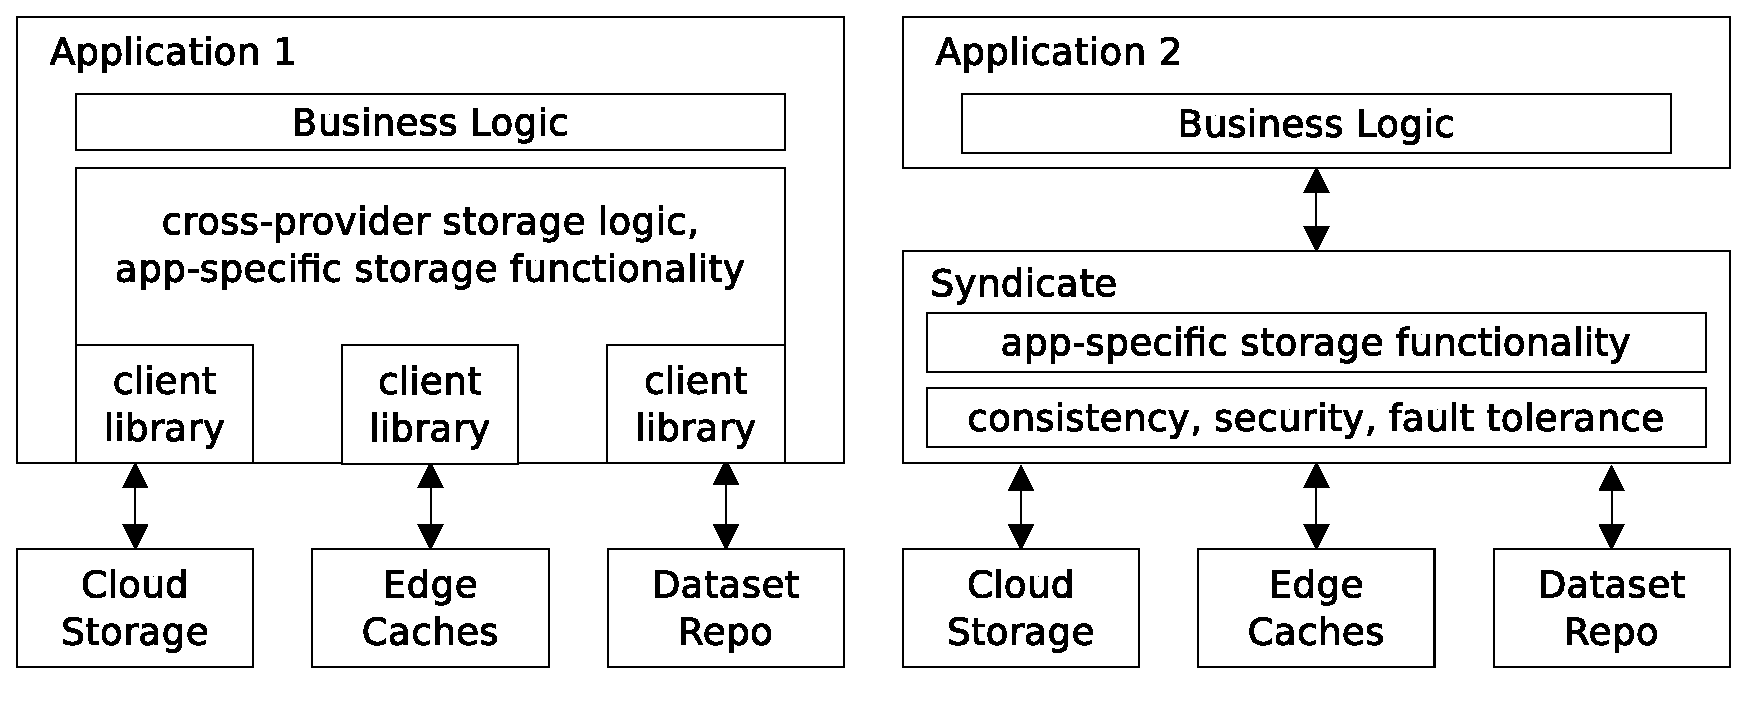
\includegraphics[width=0.5\textwidth]{figures/overview}
\caption{\it Overview of the STEAK architecture, and various data flows that must take place before Alice sends a message to Bob.  Solid-head arrows are part of the AutoKey process.  Unfilled-head arrows are part of the SMRP process.}
\label{fig:overview}
\end{figure}


In AutoKey, each user is given an account public/private key pair, a storage public/private key pair, and one or more signing public/private key pairs.  The private keys are stored encrypted with the user's password, and only decrypted when the device is running a session.  The storage and signing public keys are made available in the form of certificates signed by the account private key.  The use for each key pair is listed in Table~\ref{tab:keypairs}.

\begin{table*}[ht!]
\begin{tabular}{ | l | p{14cm} |}
\hline
\textbf{Key Pair Name} & \textbf{Usage} \\
\hline
Account key pair & Certifying and revoking other public keys. \\
Storage key pair & Sealing/unsealing and signing cloud-hosted data.  Used for message confidentiality and state CIA. \\
Signing key pair & Signing email messages and attachments.  Used for message integrity and authenticity. \\
\hline
\end{tabular}
\caption{\it Names and usages for a user`s key pairs used in STEAK`s AutoKey subsystem.}
\label{tab:keypairs}
\end{table*}


\subsubsection{Storage}
STEAK protects the contents of cloud storage from tampering by replicating cryptographic signatures.  Each file uploaded to cloud storage is sealed with the user's storage private key for confidentiality.  STEAK organizes the files into a Merkel tree, such that each directory contains the signed hash of all of its children's signed hashes.  Each hash is sealed by the storage private key, making external tampering from Mal evident.

Writing data is similar to two-phase commit.  A writer endpoint prepares to write by generating the new root signature, and replicating it to its STEAK server and all metadata repositories.  If they all authenticate and accept it, the writer uploads the data to cloud storage, and then broadcasts a signed success message.  The write completes when the STEAK server and metadata repositories acknowledge upon successful authentication.

Because reads and writes are serialized by the fact that the user does not use two endpoints simultaneously, the metadata repository only needs to store the last root signature it received.  To avoid timing out partway through writing, the endpoint splits large writes into smaller ones and commits them separately.

On read, the endpoint verifies the integrity of cloud storage by fetching the root signatures from these servers and comparing them to the one in cloud storage.  Because Mal cannot compromise all servers, and cannot compromise all channels, the reader will learn if Mal has tampered with a server if the signatures do not match.  These read and write protocols are executed by AutoKey to store trusted public keys in a tamper-evident way.

Given the threat Mal poses to the system, STEAK employs a fail-fast approach to handling storage faults.  This is because unavailability or inconsistencies discovered in publicly-hosted data (such as incorrect signatures) are assumed to be due to external interference from Mal.  This is a reasonable trade-off, because it alerts users and cloud storage operators to Mal's presence.  In practice, STEAK servers are deployed in highly-available infrastructure to reduce the risk of transient faults leading to unavailability.

Because only the user's endpoints may write to the user's cloud storage, STEAK is fundamentally a pull-based architecture.  Instead of sending data from Alice's endpoint to Bob's email server, Alice will write messages into her cloud storage, and Bob will download them later using SMRP.  This is a departure from SMTP, which we exploit to offer an ``un-send mail'' feature and to economically disincentivize spam mail by requiring the sender to pay for storage.

\subsubsection{Usability}
A user interacts with STEAK through the web browser, using the local endpoint as a web proxy.  The UI is stored as files in cloud storage and are signed by the storage private key.  This lets the endpoint verify their authenticity and integrity before serving them over the local trusted RPC channel, effectively preventing code injection attacks from Mal.

Before Alice or Bob can use STEAK, they must set up the endpoint code.  However, this can be made easy in practice (see section~\ref{sec:implementation}).  We assume in the following sections that the endpoints all run instances of the endpoint code in local VMs.

\subsection{Bootstrapping Trust}
Before Alice can use STEAK, she needs an account.  In creating one, she bootstraps AutoKey by establishing her public key and registration date with each component, populating her cloud storage with initial application state, and granting her endpoint permission to access it.  She also establishes security questions and answers to be used to recover her private key, should she forget her password.

\begin{figure}[h!]
\centering
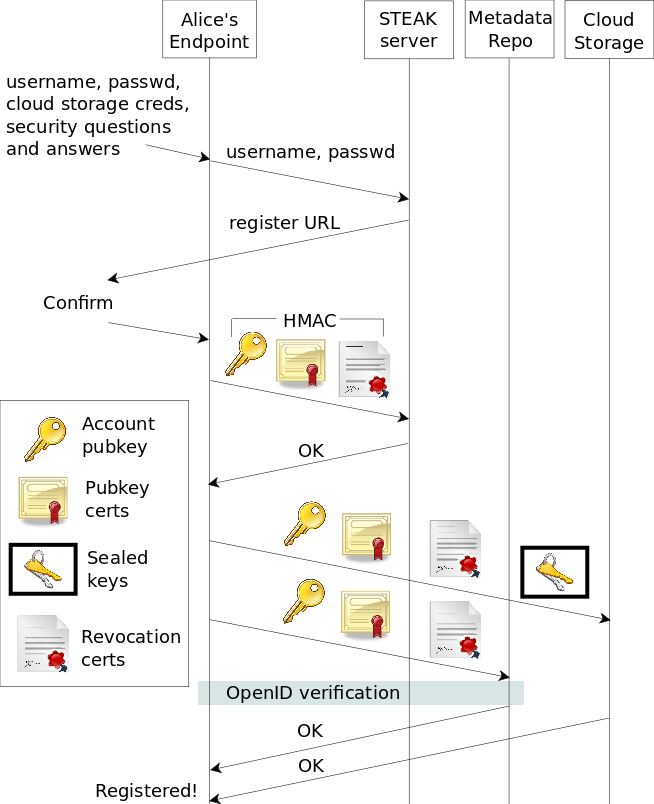
\includegraphics[width=0.5\textwidth]{figures/register}
\caption{\it The STEAK key registration protocol.}
\label{fig:register}
\end{figure}

To do so, her endpoint replicates her account public key and backs up her revocation certificate to more servers than Mal can compromise.  We assume that Mal cannot alter the behavior of the servers during the registration process; if the servers do not behave correctly, the registration fails (Figure~\ref{fig:register}).

From a usability standpoint, creating an account on the STEAK server is similar to doing so on a webmail server.  Alice begins by submitting a desired username and password to the STEAK server through the endpoint, as well as any number of hard-to-guess security questions and answers, and the identifier for an uncompromisable out-of-band channel to confirm the registration (e.g. a phone number or existing email address).  The STEAK-specific extra requirements are the authentication tokens needed to access her cloud storage, and her additional metadata repositories.

Once the information is entered, the endpoint uploads the username and password to the STEAK server, which replies with a one-time-use registration URL via the out-of-band channel (we assume that Eve cannot determine the password in this step).  Alice navigates to the URL to complete her registration.  Once Alice confirms, the STEAK server remembers iterated salted hash of the password and out-of-band channel identifier, so Eve and Mal cannot easily learn either and so Alice can use the channel identifier later to reset her password.

Once Alice's account is created on the STEAK server, the endpoint sets up her keys and certificates.  It generates her public/private key pairs, and signs the storage and signing public keys with the account private key.  It then generates revocation certificates for the account and storage keys, as well as two public certificates---one for the signing key, and one for the storage key---that contain Alice's username, the public key, the timestamp, and a nonce for uniqueness (``pubkey certs'' in Figure~\ref{fig:register}).  It signs these certificate with the account private key.

It then proceeds to replicate the account public key and certificates to each server, using the STEAK server to vouch for her.  To upload them to the STEAK server, It generates an HMAC over them using the password as the shared secret.  Once the STEAK server validates and accepts them (remembering the nonce to prevent re-register attacks), the endpoint uploads them to each metadata repository.  The endpoint authenticates to each using OpenID protocol and Alice's password, where the STEAK server acts as the OpenID provider.  The metadata repositories do not consider a revocation certificate to be in force until Alice activates it later.

The endpoint finishes by populating Alice's cloud storage with STEAK account state, using the authentication tokens she supplied at the beginning of the process.  It uploads her public key certificates as a world-readable files in cloud storage (for Bob to download later) as well as her revocation certificates and account public key (which are NOT encrypted).  It encrypts the private keys and cloud storage credentials using an authenticated symmetric key scheme, deriving symmetric keys from her salted password.  It also seals a copy of the storage private key with the answers to her security questions, so Alice can change her password without losing her data.  The endpoint uploads the security questions and sealed keys to cloud storage, seals the MACs and salts from the encryption with the password, and erases them from RAM, completing the registration and AutoKey bootstrap process.

\subsection{Session Management}
Once AutoKey is bootstrapped, Alice can use multiple endpoints to access her account transparently.  To do so, Alice simply enters her username and password, and the endpoint (via AutoKey) fetches her sealed storage private key, endpoint-specific sealed signing private key, and sealed cloud storage credentials.  If the device has never been used before, the endpoint generates a new signing key certificate and revocation certificate for it, seals the private key with the password, and distributes the certificates to the STEAK server and metadata repositories (which authenticate them with the account public key they obtained on registration).  The servers do not publish the revocation certificates until Alice signals them to do so.

Alice has the option to designate that the endpoint will be used for only one session (akin to a ``This device is public'' checkbox in webmail).  If so, the signing key will have an expiration date in the very near future, e.g. 30 minutes.

When Alice logs out or her session times out, the endpoint has AutoKey erase any secrets from RAM.  As a precaution, it also erases any data it cached data, and will erase cached data automatically if it restarts. Cached data is always sealed with one of Alice's public keys before being written to local storage, preventing Eve from breaking confidentiality via offline analysis.

\subsection{Key Distribution}
In AutoKey, Bob's endpoint must learn Alice's account, storage, and signing public keys before he can communicate with her.  Once it has them, AutoKey puts them into his cloud storage, executing the two-phase write protocol so his other endpoints can securely and automatically fetch them later.  The challenges are in obtaining them for the first time in such a way that Eve and Mal cannot trick him into learning the wrong ones, and in revoking trust in them without also being tricked.

Bob's endpoint will trust one of Alice's public keys only if AutoKey can get unanimous agreement on the key's value from each server that hosts them, and only if the key is not expired.  Similarly, AutoKey will check for an activated revocation certificate if all servers agree on the same key, and the key is different from the currently trusted key.  This strategy works under our threat model because without Alice's password, Mal is not powerful enough to send the wrong key on every channel, or change it to every server.  Bob waits for unanimous disagreement before checking for a revocation certificate to avoid Mal tricking him by activating it on one server.

While Bob trusts the keys, AutoKey periodically checks to see if it Alice's servers have changed them.  Because the account public key and storage public key do not change as often as the signing key (see the next section), it will check the account key at most once per session.  However, it will check the storage and signing public keys every time Bob sends a message to Alice.

To advertise her keys, Alice's STEAK address is a well-formed email address that indicates her username, her cloud storage provider, her STEAK server, and any metadata repositories that host her keys.  We use the character `\^{}' to separate them---for example, Alice's STEAK address might be alice\^{}cloudstorage.com\^{}keybackup.org@mail.net, indicating that her data is hosted at cloudstorage.com, her keys are replicated to keybackup.org, and her STEAK server is mail.net.  Each service makes both the keys and certificates available via canonical URLs derived from the username and the service name.  Bob's endpoint has AutoKey use TLS-secured channels with authenticated cipher suites (i.e. AES-GCM) to fetch copies from each service, in order to hedge against external tampering from Mal (but not eavesdropping from Eve).

In the event that some of Alice's services are unreachable, AutoKey continues to trust Bob's copies of Alice's public keys even if there is disagreement among the online servers.  This is to prevent Mal from weakening the system with denial-of-service attacks.  In practice, Alice's services run on highly-available infrastructure, so unreachability problems are expected to be rare and transient.

\subsection{Key Revocation}


\begin{figure}[h!]
\centering
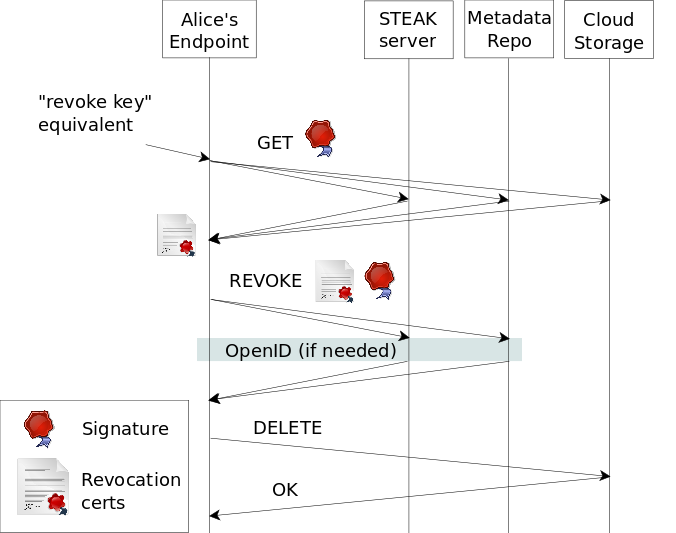
\includegraphics[width=0.5\textwidth]{figures/revoke}
\caption{\it The STEAK key revocation protocol.}
\label{fig:revoke}
\end{figure}

Inevitably, AutoKey will need to revoke Alice's keys for her.  When Alice removes access permission from a trusted endpoint device, AutoKey revokes its signing key.  When she changes or resets her password, AutoKey revokes and regenerates her keys by default because the reason for doing so may be due to a password compromise.

Revoking a signing key is a matter of activating its stored revocation certificate (Figure~\ref{fig:revoke}).  To do so, AutoKey first obtains it by downloading it from each the servers, using a request signed by the account private key.  It also gets a copy from cloud storage.  At least one of the servers will reply with the correct revocation certificate, since Mal cannot compromise all of them under our threat model.

AutoKey then re-uploads it in a signed request to the servers, indicating that the should publish it.  The servers erase the old public key certificate on successful verification, and AutoKey removes it from cloud storage.  Then, when Bob contacts Alice next, his endpoint will detect the key discrepancy, discover the revocation certificate, and stop trusting the old signing key.

If Eve compromises Alice's password, she will be able to read her incoming messages, and messages sent to others.  If Mal compromises Alice's password, she can do anything with the account.  To regain control, Alice resets her password, effectively re-registering her account and re-bootstrapping AutoKey using registration protocol described earlier (but with two small differences described below).  As before, we assume that Mal cannot alter the behavior of the servers during re-registration.

Unlike with first-time registration, the STEAK server requires Alice to submit the same out-of-band communication channel as she did before.  Also, AutoKey sets a flag while uploading new public key information to ask for a reply containing the old revocation certificate.  It also obtains the copy uploaded earlier from cloud storage, and then executes a variant of the signing key revocation protocol to publish the revocation certificates for her account and storage keys.  The only differences are that the revocation certificates will be signed by the new account key, and that the servers will additionally verify the request with OpenID to ensure that it came from Alice (the only person who knows the new password).

When Alice logs in next, her endpoint ``imports'' her old account data by unsealing it with the old storage key and re-sealing it with the new storage key.  If Alice remembers her old password, her endpoint decrypts the old storage key automatically.  If she does not, her endpoint obtains the copy of the storage key sealed with the answers to her security questions, and prompts her for them to decrypt it.

Deleting an account is similar to revoking the keys.  The only difference in the process is that no new keys are generated.

\subsection{Sending, Receiving, and Un-Sending}
Once Alice and Bob have exchanged public keys with AutoKey, they communicate with SMRP, described in this section.  In SMRP, Alice sends Bob a message by sealing it with his storage public key, uploading it to her cloud storage, and making it world-readable. Bob's endpoint downloads and decrypts it, sanitizes it, and serves it to Bob's browser for him to read. The same principle applies to attachments, which in STEAK are sent as separate files to be downloaded.  Alice makes a copy for herself in her ``sent'' folder, if desired.

If Bob expects email from Alice, he can search Alice's cloud storage for new messages and fetch them.  The UI allows him to query individual contacts for new messages.

The challenge for Bob is to discover when Alice sent him an unsolicited message.  To address this in SMRP, Bob's STEAK server acts as a notification service for new email.  Alice sends Bob's STEAK server a message metadata record, sealed with his storage public key and signed with her signing private key, that identifies herself as the sender and Bob as the recipient.  It serves as a hint to Bob that he has unsolicited mail, and tells him the message recipients, the subject, the human-readable names of the attachments, and the attachment signatures.  This information is hidden from the STEAK server to provide end-to-end message CIA, and its small size makes it easy for it to store many of them.

When Bob accesses his email, his endpoint downloads and decrypts the unread message metadata records from the server.  Each of them appear in Bob's UI as unread messages. The UI tells Bob the subject, recipients, and attachment names.  Once Bob's endpoint reads and stores the metadata records, the STEAK server is free to erase them.  

When Bob opens an unread message from Alice, his endpoint downloads, decrypts, and verifies the authenticity and integrity of Alice's message body, using the public keys obtained by AutoKey. Once verified, Bob reads it via the UI. To download an attachment, the endpoint streams it from Alice's cloud storage, verifies it, decrypts it, and delivers it to the UI as a file download.  As a performance optimization (and to assist automatic spam filtering), the endpoint prefetches message bodies as they are discovered.

Mailing lists in SMRP are treated like user accounts.  The only difference is that every participant on the list has a sealed copy of the account storage key and a personal signing key.

In SMRP, Alice can ``un-send'' a message by erasing the body and attachments from cloud storage.  This allows her to withdraw messages sent in haste, or sent accidentally to unintended people.  Bob will discover that she deleted it (i.e. he will receive a metadata record for a message that does not exist), but this may be preferable to having Bob read the entire message.  As such, once Bob obtains a message's body and attachments, his endpoint replicates them to his cloud storage by default to keep them available even if Alice deletes it later.

\subsection{Searching, Tagging, and Filtering}
Beyond sending and receiving email, webmail users expect automatic spam filtering, the ability to organize messages and conversations, and the ability to search them.  In traditional webmail systems, this functionality resides on the server.  The challenge in providing it in STEAK is in moving it to the endpoint to preserve confidentiality, but without compromising features.

Tagging messages is a matter of associating a given message with a bag of tags that Bob defines.  Bob's endpoint incrementally builds an index that pairs each tag to a list of message identifiers.  To search messages by tag, the endpoint fetches a page of the tag's index, looks up the messages, and serves them to the UI.

To search messages, the endpoint incrementally builds a search index as Bob reads them, using an off-the-shelf indexer.  The indices are updated and synchronized with cloud storage in the background as he opens and reads messages.  As a performance optimization, the endpoint lazily downloads the index by chunk they are needed by the indexer.  It caches them for the session, and asynchronously replicates modifications.

To filter messages, the endpoint uses a combination of a locally-trained classifier and sender blacklists.  Bob has the option of marking messages as spam and marking senders as spammers, in which case the endpoint feeds the message body into its local spam classifier and replicates the classifier's new model parameters to cloud storage.  This allows the classifier to be used across endpoints without revealing its parameters.  If Bob marks a contact as a spammer, AutoKey revokes trust in its public key, and the endpoint will ignore future messages from it.

Using only a local spam filter is desirable for confidentiality.  The spam classifier model parameters can leak information about the contents of the messages they have classified, so it is important that Bob's endpoint not share this information directly.  This is in contrast to webmail providers today, which learn to classify spam by monitoring many user accounts.  However, empirical tests~\cite{local-spam-filter-eval} suggest that existing local spam filters can achieve upwards of 98\% effectiveness in practice, suggesting that our strategy should not significantly impact usability if the endpoint code ships with a pre-trained classifier.

\subsection{Backwards Compatibility}
Because email is already a widely-used service, STEAK must remain backwards compatible with it to allow Alice and Bob to communicate with Charles, a user who relies on conventional email.  To do so, the STEAK server provides an SMTP/SMRP gateway that translates one protocol into the other.  The STEAK server has its own cloud storage to hold messages from Charles to serve to Alice via SMRP.  Alice's messages to Charles are automatically routed through SMTP because Charles does not have a well-formed STEAK email address.

The gateway alone does not provide CIA guarantees.  If Charles wants a limited degree of CIA, STEAK offers one of two options that require a minimal change in his workflow.  First, if Charles uses PGP already, he will send his public key and encrypted messages via SMTP.  AutoKey obtains Charles' public key automatically.  While this is less trustworthy than STEAK's approach, it is better than nothing, because Mal has only one very short window of time to alter the public key.

If Charles does not use PGP, he must first agree with Alice on a shared secret out-of-band, and assume that Mal does not compromise the STEAK server or the TLS CA server that vouches for its TLS public key.  To send her a message securely, he navigates to her STEAK server, enters the secret, and is given a webmail form for composing her a message.  When he submits his message, STEAK it available to Alice via SMRP.

When Alice replies via SMRP, the STEAK server sends Charles a URL instead of the message body.  When opened, the STEAK server gives him a specially-crafted HTML page that contains Alice's ciphertext, a decryption algorithm in Javascript, and a secret submission form.  When Charles enters the secret, the page decrypts the message for him.

\section{Implementation}

The individual technologies needed to implement STEAK already exist.  For storage, STEAK relies on Syndicate to provide an abstraction layer over storage providers while implementing common consistency, integrity, authenticity, and authorization semantics.  For running the endpoint code, STEAK relies on now-ubiquitous virtual machine technology to achieve portability and isolation from the browser and underlying OS.

The two usability challenges to overcome are setting up the endpoint VM and getting access to the user’s cloud storage.  To address the former, we deliver endpoint code as an “app” that the user installs via a device-specific app store.  Once installed, it does not have to be accessed directly, and the app store will keep it up-to-date.  We believe users are already used to installing software from app stores, and thus we do not believe this extra step poses a significant usability barrier.

Our endpoint’s runtime requirements are flexible.  While a full-blown virtual machine is sufficient, the endpoint can also run in an OS container, a user-mode Linux~\cite{usermode-linux} instance, or a Portable Native Client (PNaCl)~\cite{pnacl} browser plugin.  Our prototype supports all but the last option, which is under development.

We leverage Syndicate to make it easy to access cloud storage, and to simplify our storage layer’s implementation.  To set up STEAK, the endpoint and Syndicate execute a protocol similar to OpenID whereby Alice authorizes STEAK to create and access a Syndicate volume.  The metadata repository implementation employs a similar strategy.

Regarding deployments, a STEAK server is meant to serve an organization.  Because it can read sender email addresses and source IP addresses, it employs techniques similar to those used in SMTP to rate-limit and black/whitelist external malicious users.  For SMRP clients, the server additionally verifies the message metadata record signature before accepting the request, and blocks senders who do not have known public keys.  The server deals with malicious traffic on the SMTP gateway using conventional techniques.

Regarding spam, since Bob can be expected to check his account frequently (once per day), it is unlikely that his message metadata records on his STEAK server will consume too much space.  If space becomes a concern, the STEAK server can opt to remember only the unique set of senders, in which case Bob will scan their cloud storage accounts for the messages at the cost of latency.

To enhance spam filtering, we are investigating the feasibility of privacy-preserving data mining, to allow many users to train a shared spam classifier.  One possible solution is a distributed privacy-preserving Na\"{i}ve Bayes classifier~\cite{privacy-preserving-naive-bayes}.

Key plaque is a known problem with key servers.  Metadata repositories prevent it by periodically querying the issuer's STEAK server for the key, and automatically erasing certificates with built-in expiration dates.

\subsection{Prototype}
Our prototype is in an early alpha state, but is under active development.  The endpoint and server are implemented as daemons in Python, with 6,000 and 1,000 lines of code respectively.  The UI is implemented with Google Web Toolkit, and contains about 2,000 lines of Java. We use the PyCrypto package for cryptography, and rely on Syndicate’s Metadata Service as a metadata repository.  We are in the process of integrating the logic for handling attachments, mailing lists, searching, and filtering.

The STEAK server and metadata repository will be compatible with multiple PaaS providers, to allow them to horizontally scale to support large organizations.  Users will have the option to write public keys and certificates to one or more cryptocurrency blockchains, greatly increasing the number of servers Mal must compromise to change it.

\section{Preliminary Evaluation}
\label{sec:evaluation}

We have deployed our \MS\ on Google AppEngine~\cite{google-appengine},
and our Replica and Acquisition \SGs\ on PlanetLab~\cite{planetlab}.
They use a CDN running on VICCI~\cite{vicci} based on 
CoBlitz~\cite{coblitz}, and use Amazon S3 to make data durable.  We are in the
process of gathering large-scale usage data.

\Syndicate's performance is partially determined by the 
underlying providers.  Our microbenchmarks indicate that User \SG\
and Replica \SG\ contribute a small constant-factor overhead on top of directly 
uploading data to cloud storage and downloading data from the CDN.

\Syndicate's main performance bottlenecks are in reading consistent data
in the face of writes, and in handling many writes on the same object.
The costs for consistency come from re-synchronizing
stale metadata and missing overwritten blocks in the cache.  A preliminary
test with PlanetLab nodes shows that half of metadata refreshes take less than 200 milliseconds, and 
90\% take less than 300 ($n=300$).

Another early consistency evaluation shows that the time required to read an object
is linear in the fraction of blocks overwritten,
with $r^2=0.983$ for the median read times and $r^2=0.939$ for the 90\% percentile read
times ($n=300$).  The nodes read a 100-block object in increments of 10 blocks,
with a 60KB block size (i.e. the size of a large gene sequence from GenBank).
Blocks were downloaded sequentially, but we expect similar results if the 
blocks are downloaded in parallel.  This represents the expected performance 
profile for reading with ongoing writes, as well as for distributing new certificates and \SG\ code.

The performance costs in writing to the same object come from write serialization in the \MS.
In an experiment where 300 nodes wrote metadata to the same object,
50\% of \MS\ responses take less than 1500 milliseconds, and 90\% take less than 2350 milliseconds.
The \MS\ operations are I/O bound in local tests, and according to Google AppEngine's internal measurements, at
most 250 milliseconds are spent accessing the datastore and performing TLS negotiation.
This suggests most of the latency comes from the platform's internal request buffering,
including waiting for new front-end instances to spin up.  As such, we believe this data
is indicative of the \MS's performance under load.  We are working on preventing the 
platform from contributing so much overhead.

We are also in the process of evaluating the User \SG's ability to handle many concurrent
writes, as well as its ability to shed load to other User \SGs.
We anticipate that a loaded User \SG\ will naturally distribute coordinator responsibility to
heavy writers, since statistically their writes are most likely to fail first.

The take-away from our preliminary tests is that composing providers to reap their aggregate utility benefits is feasible 
in practice. They -- not \Syndicate\ -- are the limiting factor in performance, so it is to the developer's
advantage to select providers with the best cost/performance trade-off while using \Syndicate.
\section{Related Work}

Since inception of SMTP little had been done with respect to mail transport
protocol. Most of these works argue that design of SMTP incentivize SPAM as it
gives no control over receiver to what he gets in his inbox. It has also been
argued that in general push based architectures/protocols have a higher tendency
to attract unwanted traffic\cite{PushVsPull}. Therefore these works suggest a
pull based approach to email instead of the push based approach used by SMTP. 

DMTP (Differentiated Message Delivery Protocol) \cite{dtmp} is a protocol that
forces sender to store email in his own storage before recipient reads it into
his inbox unless the sender is known in advance. Only emails sent by senders
knowns to the recipient will be stored in recipient's mail box. Due to this
approach DMTP eliminates economies of scale and increases accountability of
SPAM.

In 2000 Internet Mail 2000 \cite{im2k} was proposed by Daniel J. Bernstein,
which shifts the responsibility of mail storage from recipient to sender through
a pull based approach that replaces SMTP which is analogous to conventional
smail mail. Original IM 2000 proposal does not specify mechanisms such as how
recipients should be notified, how messages should be downloaded etc. StubMail
\cite{stubmail} is an implementation of IM 2000, with StubMail sender uploads
the email to a permanently connected outbox (storage) and sends a UDP
notification to the recipient’s mail service provider as an RSS feed. Similar to
DMTP this implementation also shifts storage responsibility from recipient to
sender discouraging SPAMers. StubMail uses either HTTP \cite{HTTP-RFC} or 
SMTP\cite{SMTP-RFC} to upload mail to the outgoing storage, message notifications 
were sent over UDP to eliminate possibility of DoS attacks that could happen with 
TCP. HTMP (Hypertext Mail Protocol)\cite{htmp} too is based on IM 2000 and uses 
HTTP as a transport utilizing its’ PUT, GET and DELETE methods to handle email. 
In all of these designs email addresses of the sender and the receiver have to be 
exchanged out of band since receiver cannot receive emails if receiver does not 
know the location of sender’s mail OutBox.

However none of these designs were adopted as a main stream email protocol, this
could have been largely due to wide adoption of SMTP and availability of free
webmail services like GMail\cite{GMail}. At the time of inception there was no 
incentive in pushing storage responsibility to end - user when free webmail 
systems  were readily available with Gigabytes of storage. However during the 
last few years webmail users have become more conscious about privacy and fully 
aware of the fact that free storage comes at the cost of either being spied by 
the  government or becoming a target of an advertising campaign. On the other 
hand high availability online storages systems have become feasible enough for 
individual users through cloud storage services like Amazon S3\cite{AWS-S3},
Dropbox\cite{DRPBX} etc. Therefore current technology and circumstances calls 
for a new mail transfer protocol that follows IM 2000 but accompanying novel 
mechanisms with respect to storage and privacy. In addition users are also keen 
on having full control over their content stored in the cloud storage and ability 
to move their data across different cloud storage providers. On the other hand by 
allowing users to plug-in their own cloud storage webmail services can liberate 
themselves from the burden of developing and maintaining high performance backend 
storage systems optimized for serving email.



\section{Conclusion}

We have presented Syndicate, a distributed read-write filesystem
that uses a CDN to achieve high read performance despite any performance
shortcomings of the data's underlying storage mechanisms.  Syndicate can
leverage any CDN to drive file data delivery between its clients, as long 
as it meets a few simple design requirements.  Syndicate's read performance
is dependent on the underlying CDN implementation, which is the limiting
factor in the number of bytes distributed to clients.  However, by depending
on a CDN to drive data performance, Syndicate assumes its data availability,
read throughput, and network capacity properties.

Syndicate overcomes the immutability assumptions a CDN makes about 
the content it caches through the use of a central metadata server
that observes all metadata operations.  Syndicate achieves close-to-open 
file consistency by versioning file URLs and reading from the most
recently written version of the file.  Syndicate delivers low-latency
write performance by storing written data locally and asynchronously
informing the metadata server of metadata changes.  Finally, Syndicate
 efficiently exposes large hierarchies of data, which many clients
read efficiently by leverage the CDN to its fullest potential.



%\comment{
\section{Acknowledgements}

We wish to thank Sapan Bhatia and Andy Bavier for their assistance on technical matters
such as preparing VICCI slices to run Hypercache and FUSE filesystems, as well as providing
guidance on building back-end on Hypercache to interface with public slice-federation architectures
such as VICCI.  We also wish to thank G\"{u}rer \"{O}zen, \c{C}a\u{g}lar Onur, Baris Metin, and Marc Fiuczynski
for their technical assistance in configuring and deploying Hypercache on VICCI.  Additionally, we
wish to thank Verivue, Inc. for allowing us to run their CDN implementation on a publicly-accessible
testbed.
}



{\footnotesize \bibliographystyle{acm}
{\bibliography{bibdata}}

\end{document}








